\documentclass[author-year, 8pt, 3p]{elsarticle} %review=doublespace preprint=single 5p=2 column
\usepackage{amsmath, amsfonts, amssymb}  % extended mathematics

% My package additions
\usepackage[hyphens]{url}
\usepackage{lineno} % add 
%\linenumbers % turns line numbering on 
\bibliographystyle{elsarticle-harv}
\biboptions{sort&compress} % For natbib
\usepackage{graphicx}
\usepackage{booktabs} % book-quality tables

%% Redefines the elsarticle footer
\makeatletter
\def\ps@pprintTitle{%
 \let\@oddhead\@empty
 \let\@evenhead\@empty
 \def\@oddfoot{\it \hfill\today}%
 \let\@evenfoot\@oddfoot}
\makeatother

% A modified page layout
\textwidth 6.75in
\oddsidemargin -0.15in
\evensidemargin -0.15in
\textheight 9in
\topmargin -0.5in


\usepackage{microtype}

%\usepackage{listings}
%\lstnewenvironment{code}{\lstset{language=Haskell,basicstyle=\small\ttfamily}}{}


\setlength{\parindent}{0pt}
\setlength{\parskip}{6pt plus 2pt minus 1pt}


%%% Syntax Highlighting for code  %%%
%%% Adapted from knitr book %%% 
\usepackage{fancyvrb}
\DefineVerbatimEnvironment{Highlighting}{Verbatim}{commandchars=\\\{\}}
% Add ',fontsize=\small' for more characters per line
\newenvironment{Shaded}{}{}
\newcommand{\KeywordTok}[1]{\textcolor[rgb]{0.00,0.44,0.13}{\textbf{{#1}}}}
\newcommand{\DataTypeTok}[1]{\textcolor[rgb]{0.56,0.13,0.00}{{#1}}}
\newcommand{\DecValTok}[1]{\textcolor[rgb]{0.25,0.63,0.44}{{#1}}}
\newcommand{\BaseNTok}[1]{\textcolor[rgb]{0.25,0.63,0.44}{{#1}}}
\newcommand{\FloatTok}[1]{\textcolor[rgb]{0.25,0.63,0.44}{{#1}}}
\newcommand{\CharTok}[1]{\textcolor[rgb]{0.25,0.44,0.63}{{#1}}}
\newcommand{\StringTok}[1]{\textcolor[rgb]{0.25,0.44,0.63}{{#1}}}
\newcommand{\CommentTok}[1]{\textcolor[rgb]{0.38,0.63,0.69}{\textit{{#1}}}}
\newcommand{\OtherTok}[1]{\textcolor[rgb]{0.00,0.44,0.13}{{#1}}}
\newcommand{\AlertTok}[1]{\textcolor[rgb]{1.00,0.00,0.00}{\textbf{{#1}}}}
\newcommand{\FunctionTok}[1]{\textcolor[rgb]{0.02,0.16,0.49}{{#1}}}
\newcommand{\RegionMarkerTok}[1]{{#1}}
\newcommand{\ErrorTok}[1]{\textcolor[rgb]{1.00,0.00,0.00}{\textbf{{#1}}}}
\newcommand{\NormalTok}[1]{{#1}}
\usepackage{enumerate}
\usepackage{ctable}
\usepackage{float}

% This is needed because raggedright in table elements redefines \\:
\newcommand{\PreserveBackslash}[1]{\let\temp=\\#1\let\\=\temp}
\let\PBS=\PreserveBackslash
\usepackage[normalem]{ulem}
\newcommand{\textsubscr}[1]{\ensuremath{_{\scriptsize\textrm{#1}}}}

% Configure hyperlinks package
\usepackage[breaklinks=true,linktocpage,pdftitle={Treebase: An R package for discovery, access and manipulation of online
                                                  phylogenies},pdfauthor={},colorlinks]{hyperref}
\hypersetup{breaklinks=true, pdfborder={0 0 0}}

% Pandoc toggle for numbering sections (defaults to be off)
\setcounter{secnumdepth}{0}


\VerbatimFootnotes % allows verbatim text in footnotes

% Pandoc header



\begin{document}
\begin{frontmatter}
  \title{Treebase: An R package for discovery, access and manipulation of online
         phylogenies}
  \author[cpb]{Carl Boettiger\corref{cor1}}
  \ead{cboettig@ucdavis.edu}
  \cortext[cor1]{Corresponding author}
  \address[cpb]{Center for Population Biology, University of California, Davis, California 95616}
  \author[stats]{Duncan Temple Lang}
  \address[stats]{Department of Statistics, University of California, Davis, California 95616}
 \end{frontmatter}


\begin{enumerate}[1.]
\item
  The TreeBASE portal is an important and rapidly growing repository of
  phylogenetic data. The R statistical environment has also become a
  primary tool for applied phylogenetic analyses across a range of
  questions, from comparative evolution to community ecology to
  conservation planning.
\item
  We have developed \texttt{treebase}, an open-source software package
  (freely available from
  \href{http://cran.r-project.org/web/packages/treebase}{http://cran.r-project.org/web/packages/treebase})
  for the R programming environment, providing simplified,
  \emph{programmatic} and interactive access to phylogenetic data in the
  TreeBASE repository.
\item
  We illustrate how this package creates a bridge between the TreeBASE
  repository and the rapidly growing collection of R packages for
  phylogenetics that can reduce barriers to discovery and integration
  across phylogenetic research.
\item
  We show how the \texttt{treebase} package can be used to facilitate
  replication of previous studies and testing of methods and hypotheses
  across a large sample of phylogenies, which may help make such
  important reproducibility practices more common.
\end{enumerate}
\paragraph{Keywords}

R, software, API, TreeBASE, database, programmatic, workflow

\section{Introduction}

Applications that use phylogenetic information as part of their analyses
are becoming increasingly central to both evolutionary and ecological
research. The exponential growth in genetic sequence data available for
all forms of life has driven rapid advances in the methods that can
infer the phylogenetic relationships and divergence times across
different taxa (Huelsenbeck and Ronquist 2001; Stamatakis 2006; Drummond
and Rambaut 2007). The product of one field has become the raw data of
the next. Unfortunately, while the discipline of bioinformatics has
emerged to help harness and curate the wealth of genetic data with
cutting edge computer science, statistics, and Internet technologies,
its counterpart in evolutionary informatics remains ``scattered, poorly
documented, and in formats that impede discovery and integration'' (Parr
et al. 2011). Our goal in developing the \texttt{treebase} package is to
provide steps to reduce these challenges through programmatic and
interactive access between the repositories that store this data and the
software tools commonly used to analyse them.

The R statistical environment (R Development Core Team 2012) has become
a dominant platform for researchers using phylogenetic data to address a
rapidly expanding set of questions in ecological and evolutionary
processes. These methods include, but are not limited to, ancestral
state reconstruction (Paradis 2004; Butler and King 2004),
diversification analysis (Paradis 2004; Rabosky 2006; Harmon et al.
2008), identifying trait dependent speciation and extinction rates,
(Fitzjohn 2010; Goldberg, Lancaster, and Ree 2011; Stadler 2011b),
quantifying the rate and tempo of trait evolution (Butler and King 2004;
Harmon et al. 2008; Eastman et al. 2011), identifying evolutionary
influences and proxies for community ecology (Webb, Ackerly, and Kembel
2008; Kembel et al. 2010), connecting phylogeny data to climate patterns
(Warren, Glor, and Turelli 2008; Evans et al. 2009), and simulation of
speciation and character evolution (Harmon et al. 2008; Stadler 2011a;
Boettiger, Coop, and Ralph 2012), as well as various manipulations and
visualizations of phylogenetic data (Paradis 2004; Schliep 2010;
Jombart, Balloux, and Dray 2010; Revell et al. 2011). A more
comprehensive list of R packages by analysis type is available on the
phylogenetics taskview,
\href{http://cran.r-project.org/web/views/Phylogenetics.html}{http://cran.r-project.org/web/views/Phylogenetics.html}.
Libraries and packages are developed for use in other general purpose
programming environments and languages, including Java (Maddison and
Maddison 2011), MATLAB (Blomberg, Garland, and Ives 2003) and Python
(Sukumaran and Holder 2010) and online interfaces (Martins 2004). In
particular, the Bio::Phylo toolkit (Vos et al. 2011) not only provides a
PERL implementation of some of the common phylogenetic simulation and
visualization tools found in these R libraries, but can already provide
programmatic access to TreeBASE. Our goal is to bring similar
functionality to the larger suite of applied phylogenetics methods and
user in the R community.

TreeBASE (\href{http://treebase.org}{http://treebase.org}) is an online
repository of phylogenetic data (e.g.~trees of species, populations, or
genes) that have been published in a peer-reviewed academic journal,
book, thesis or conference proceedings (Sanderson et al. 1994; Morell
1996). The database can be searched through an online interface which
allows users to find a phylogenetic tree from a particular publication,
author or taxa of interest. TreeBASE provides an application programming
interface (API) that lets computer applications make queries to the
database, known as PhyloWS (Vos et al. 2010). Our \texttt{treebase}
package uses this API to create a direct link between this data and the
R environment. This has several immediate and important benefits:

\begin{enumerate}[1.]
\item
  \emph{Data discovery.} Users can leverage the rich, higher-level
  programming environment provided by the R environment to better
  identify data sets appropriate for their research by iteratively
  constructing queries for datasets that match appropriate metadata
  requirements.
\item
  \emph{Programmatic data access.} Many tasks that are theoretically
  made possible by the creation of the Web-base interface to the
  TreeBASE repository are not pursued because they would be too
  laborious for an exploratory analysis. The ability to use programmatic
  access across data sets to automatically download and perform a
  reproducible and systematic analysis using the rich set of tools
  available in R opens up new avenues for research.
\item
  \emph{Automatic updating}. The TreeBASE repository is expanding
  rapidly. The scriptable nature of analyses run with our
  \texttt{treebase} package means that a study can be rerun on the
  latest version of the repository without additional effort but with
  potential new information.
\end{enumerate}
\subsection{Programmatic Web Access}

The TreeBASE repository makes data accessible via Web queries through a
RESTful (REpresentational State Transfer) interface, which supplies
search conditions in the address URL. The repository returns the
requested data in XML (extensible markup language) format, conforming to
the RSS1.0 standard. Because the RSS1.0 format allows the search results
to also be viewed in a human-readable format in common browsers such as
Safari and Firefox, the \texttt{treebase} package echoes this URL to the
console, so that the user can explore the results in the browser as
well. The \texttt{treebase} package uses the \texttt{RCurl} package
(Temple Lang 2012a) to make queries over the Web to the repository, and
the \texttt{XML} package (Temple Lang 2012b) to parse the Web page
returned by the repository into meaningful R data objects. While these
querying and parsing functions comprise most of the code provided in the
\texttt{treebase} package, they are hidden from the end user who can
interact with these rich data retrieval and manipulation tools to access
data from these remote repositories in much the same way as data locally
available on the users hard-disk.

While the TreeBASE repository provides phylogenies in both the
traditional Nexus file format and the more data-rich NeXML format (Vos
et al. 2012), none of the R packages currently available for
phylogenetic research are positioned to read these NeXML files. The next
version of the \texttt{treebase} package will provide extraction of
metadata information from the NeXML through XML parsing.

\subsection{Basic queries}

The \texttt{treebase} package allows these queries to be made directly
from R. Programmatic access also allows a user to go beyond the
utilities of the Web interface, constructing more complicated queries
and allowing the user to maintain a record of the commands used to
collect their data as an R script. Scripting the data-gathering process
helps reduce errors and assists in replicating the analysis later,
either by the authors or other researchers (Peng 2011).

The \texttt{search\_treebase} function forms the base of the
\texttt{treebase} package. Table 1 lists each of the types of queries
available through the \texttt{search\_treebase} function. This list can
also be found in the function documentation through the R command
\texttt{?search\_treebase}.\\Any of the queries available on the Web
interface can now be made directly from R, including downloading and
importing a phylogeny into the R session. For instance, one can search
for phylogenies containing dolphin taxa, ``Delphinus,'' or all
phylogenies submitted by a given author, ``Huelsenbeck'' using the R
commands

\begin{Shaded}
\begin{Highlighting}[]
    \KeywordTok{search_treebase}\NormalTok{(}\StringTok{"Delphinus"}\NormalTok{, }\DataTypeTok{by=}\StringTok{"taxon"}\NormalTok{)}
    \KeywordTok{search_treebase}\NormalTok{(}\StringTok{"Huelsenbeck"}\NormalTok{, }\DataTypeTok{by=}\StringTok{"author"}\NormalTok{)}
\end{Highlighting}
\end{Shaded}
The \texttt{search\_treebase} function returns the matching phylogenies
as an R object, ready for analysis. The package documentation provides
many examples of possible queries.

\ctable[caption = Queries available in \texttt{search\_treebase}. The
first argument is the keyword used in the query such as an author's name
and the second argument indicates the type of query (\emph{i.e.}
``author'')., pos = H, center, botcap]{ll}
{% notes
}
{% rows
\FL
Search ``by='' & PURPOSE
\ML
abstract & search terms in the publication abstract
\\\noalign{\medskip}
author & match authors in the publication
\\\noalign{\medskip}
subject & Matches in the subject terms
\\\noalign{\medskip}
doi & The unique object identifier for the publication
\\\noalign{\medskip}
ncbi & NCBI identifier number for the taxon
\\\noalign{\medskip}
kind.tree & Kind of tree (Gene tree, species tree, barcode tree)
\\\noalign{\medskip}
type.tree & Type of tree (Consensus or Single)
\\\noalign{\medskip}
ntax & Number of taxa in the matrix
\\\noalign{\medskip}
quality & A quality score for the tree, if it has been rated.
\\\noalign{\medskip}
study & Match words in the title of the study or publication
\\\noalign{\medskip}
taxon & Taxon scientific name
\\\noalign{\medskip}
id.study & TreeBASE study ID
\\\noalign{\medskip}
id.tree & TreeBASE's unique tree identifier (Tr.id)
\\\noalign{\medskip}
id.taxon & Taxon identifier number from TreeBase
\\\noalign{\medskip}
tree & The title for the tree
\LL
}

\subsection{Accessing all phylogenies}

For certain applications, a user may wish to download all the available
phylogenies from TreeBASE. Using the \texttt{cache\_treebase} function
allows a user to download a local copy of all trees. Because direct
database dumps are not currently available from treebase.org, this
function has intentional delays to avoid overtaxing the TreeBASE
servers, and should be allowed a full day to run.

\begin{Shaded}
\begin{Highlighting}[]
\NormalTok{treebase <- }\KeywordTok{cache_treebase}\NormalTok{()}
\end{Highlighting}
\end{Shaded}
Users should still be mindful that these servers are a shared community
resource and not place many queries at once. Users running large jobs
should consider joining the TreeBASE mailing list
(\href{http://sourceforge.net/mailarchive/forum.php?forum\_name=treebase-users}{http://sourceforge.net/mailarchive/forum.php?forum\_name=treebase-users})
to discuss such queries ahead of time. When query

Once run, the cache is saved compactly in memory where it can be easily
and quickly restored. For convenience, the \texttt{treebase} package
comes with a copy already cached, which can be loaded into memory.

\begin{Shaded}
\begin{Highlighting}[]
\KeywordTok{data}\NormalTok{(treebase)}
\end{Highlighting}
\end{Shaded}
The cache included in the package will be updated during major package
revisions. The timestamp of the cache provided can be viewed in the help
file for the data object using the command \texttt{?treebase} (Current
cache is May 14, 2012). All queries from \texttt{metadata()} and
\texttt{search\_treebase()} are run against the current online version
of the database.

All of the examples shown in this manuscript are run as shown using the
\texttt{knitr} package for authoring dynamic documents (Xie 2012), which
helps ensure the results shown are reproducible. These examples can be
updated by copying and pasting the code shown into the R terminal, or by
recompiling the entire manuscript from the source files found on the
development Web page for the TreeBASE package,
\href{https://github.com/ropensci/treebase}{github.com/ropensci/treebase}.
Data was accessed to produce the examples shown on Thu Aug 9 10:51:51
2012.

\section{Data discovery in TreeBASE}

Data discovery involves searching for existing data that meets certain
desired characteristics. Such searches take advantage of metadata --
summary information describing the data entries provided in the
repository. The Web repository uses separate interfaces (APIs) to access
metadata describing the publications associated with the data entered,
such as the publisher, year of publication, etc., and a different
interface to describe the metadata associated with an individual
phylogeny, such as the number of taxa or the kind of tree (\emph{e.g.}
gene tree versus species tree). The \texttt{treebase} package can query
these individual sources of metadata separately, but this information is
most powerful when used in concert -- allowing the construction of
complicated searches that cannot be automated through the Web interface.
The \texttt{metadata} function updates a list of all available metadata
from both APIs and returns this information as an R \texttt{data.frame}.

\begin{Shaded}
\begin{Highlighting}[]
\NormalTok{meta <- }\KeywordTok{metadata}\NormalTok{()}
\end{Highlighting}
\end{Shaded}
From the number of rows of the metadata list we see that there are
currently 3164 published studies in the database. The field columns
provided by \texttt{metadata} are listed in Table II.

\ctable[caption = Columns of metadata available from the
\texttt{metadata} function, pos = H, center, botcap]{ll}
{% notes
}
{% rows
\FL
metadata field & description
\ML
Study.id & TreeBASE study ID
\\\noalign{\medskip}
Tree.id & TreeBASE's unique tree identifier
\\\noalign{\medskip}
kind & Kind of tree (Gene tree, species tree, barcode tree)
\\\noalign{\medskip}
type & Type of tree (Consensus or Single)
\\\noalign{\medskip}
quality & A quality score for the tree, if it has been rated.
\\\noalign{\medskip}
ntaxa & Number of taxa in the matrix
\\\noalign{\medskip}
date & Year the study was published
\\\noalign{\medskip}
author & First author in the publication
\\\noalign{\medskip}
title & The title of the publication
\LL
}

Metadata can also be used to reveal trends in the data deposition which
may be useful in identifying patterns or biases in research or emerging
potential types of data. As a simple example, we look at trends in the
submission patterns of publishers over time:

\begin{Shaded}
\begin{Highlighting}[]
    \NormalTok{date <- meta[[}\StringTok{"date"}\NormalTok{]] }
    \NormalTok{pub <- meta[[}\StringTok{"publisher"}\NormalTok{]]}
\end{Highlighting}
\end{Shaded}
Many journals have only a few submissions, so we will label any not in
the top ten contributing journals as ``Other'':

\begin{Shaded}
\begin{Highlighting}[]
    \NormalTok{topten <- }\KeywordTok{sort}\NormalTok{(}\KeywordTok{table}\NormalTok{(pub), }\DataTypeTok{decreasing=}\OtherTok{TRUE}\NormalTok{)[}\DecValTok{1}\NormalTok{:}\DecValTok{10}\NormalTok{]}
    \NormalTok{meta[[}\StringTok{"publisher"}\NormalTok{]] <- }\KeywordTok{as.character}\NormalTok{(meta[[}\StringTok{"publisher"}\NormalTok{]])}
    \NormalTok{meta[[}\StringTok{"publisher"}\NormalTok{]][!(pub %in% }\KeywordTok{names}\NormalTok{(topten))] <- }\StringTok{"Other"}
    \NormalTok{meta[[}\StringTok{"publisher"}\NormalTok{]] <- }\KeywordTok{as.factor}\NormalTok{(meta[[}\StringTok{"publisher"}\NormalTok{]])}
\end{Highlighting}
\end{Shaded}
We plot the distribution of publication years for phylogenies deposited
in TreeBASE, color coding by publisher in Figure 1.

\begin{Shaded}
\begin{Highlighting}[]
\KeywordTok{library}\NormalTok{(ggplot2) }
\KeywordTok{library}\NormalTok{(reshape2)}
\NormalTok{df <- }\KeywordTok{acast}\NormalTok{(meta, date ~ publisher, }\DataTypeTok{value.var=}\StringTok{'publisher'}\NormalTok{, length)}
\NormalTok{df <- }\KeywordTok{melt}\NormalTok{(df, }\DataTypeTok{varnames=}\KeywordTok{c}\NormalTok{(}\StringTok{"date"}\NormalTok{, }\StringTok{"publisher"}\NormalTok{))}
\KeywordTok{ggplot}\NormalTok{(df) + }\KeywordTok{geom_area}\NormalTok{(}\KeywordTok{aes}\NormalTok{(}\DataTypeTok{x=}\NormalTok{date,}\DataTypeTok{y=}\NormalTok{value, }\DataTypeTok{fill =} \NormalTok{publisher)) }
\end{Highlighting}
\end{Shaded}
\begin{figure}[htbp]
\centering
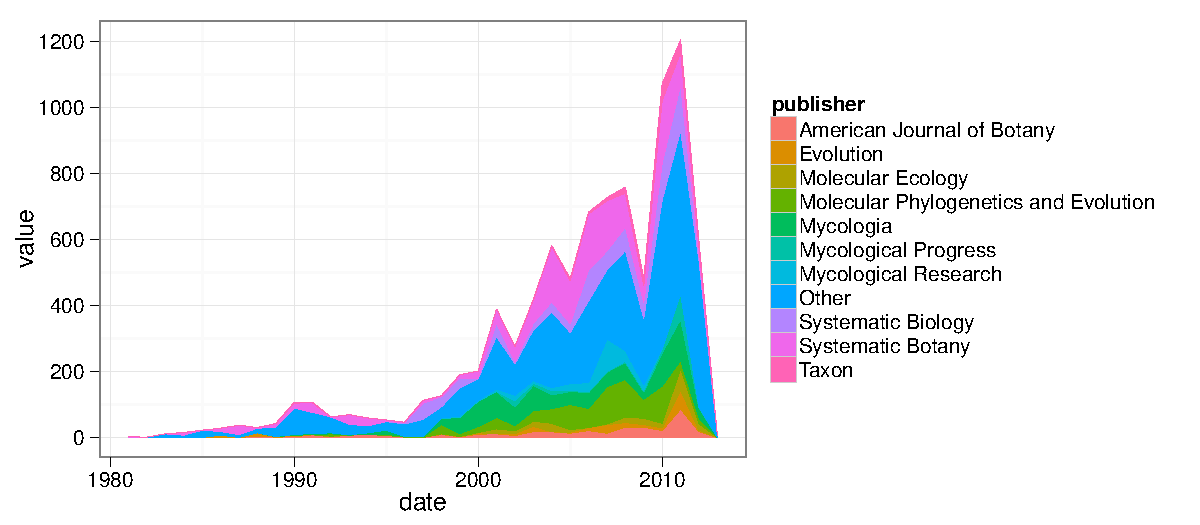
\includegraphics{figure1.pdf}
\caption{Histogram of publication dates by year, with the code required
to generate the figure.}
\end{figure}

Typically we are interested in the metadata describing the phylogenies
themselves rather than just in the publications in which they appeared.
Phylogenetic metadata includes features such as the number of taxa in
the tree, a quality score (if available), kind of tree (gene tree,
species tree, or barcode tree) or whether the phylogeny represents a
consensus tree from a distribution or just a single estimate.

Even simple queries can illustrate the advantage of interacting with
TreeBASE data through an R interface has over the Web interface. A Web
interface can only perform the tasks built in by design. For instance,
rather than performing six separate searches to determine the number of
consensus vs single phylogenies available for each kind of tree, we can
construct a 2 by 2 table with a single line of code:

\begin{Shaded}
\begin{Highlighting}[]
\KeywordTok{table}\NormalTok{(meta[[}\StringTok{"kind"}\NormalTok{]], meta[[}\StringTok{"type"}\NormalTok{]])}
\end{Highlighting}
\end{Shaded}
\begin{table}[ht]
\begin{center}
\begin{tabular}{rrr}
  \hline
 & Consensus & Single \\ 
  \hline
Barcode Tree &   1 &   4 \\ 
  Gene Tree &  65 & 134 \\ 
  Species Tree & 2863 & 5857 \\ 
   \hline
\end{tabular}
\end{center}
\end{table}

\section{Reproducible computations}

Reproducible research has become a topic of increasing interest in
recent years, and facilitating access to data and using scripts that can
replicate analyses can help lower barriers to the replication of
statistical and computational results (Schwab, Karrenbach, and Claerbout
2000; Gentleman and Temple Lang 2004; Peng 2011). The \texttt{treebase}
package facilitates this process, as we illustrate in a simple example.

Consider the shifts in speciation rate identified by Derryberry et al.
(2011) on a phylogeny of ovenbirds and treecreepers. We will seek to not
only replicate the results the authors obtained by fitting the models
provided in the R package \texttt{laser} (Rabosky 2006), but also
compare them against methods presented in Stadler (2011b) and
implemented in the package \texttt{TreePar}, which permits speciation
models that were not available to Derryberry et al. (2011) at the time
of their study.

\subsection{Obtaining the tree}

The most expedient way to identify the data uses the digital object
identifier (doi) at the top of most articles, which we use in a call to
the \texttt{search\_treebase} function, such as

\begin{Shaded}
\begin{Highlighting}[]
\NormalTok{results <- }\KeywordTok{search_treebase}\NormalTok{(}\StringTok{"10.1111/j.1558-5646.2011.01374.x"}\NormalTok{, }\StringTok{"doi"}\NormalTok{) }
\end{Highlighting}
\end{Shaded}
The search returns a list, since some publications can contain many
trees. In this case our phylogeny is in the only element of the list.

Having imported the phylogenetic tree corresponding to this study, we
can quickly replicate their analysis of which diversification process
best fits the data. These steps can be easily implemented using the
phylogenetics packages we have just mentioned.

For instance, we can calculate the branching times of each node on the
phylogeny,

\begin{Shaded}
\begin{Highlighting}[]
\NormalTok{bt <- }\KeywordTok{branching.times}\NormalTok{(results[[}\DecValTok{1}\NormalTok{]])}
\end{Highlighting}
\end{Shaded}
and then begin to fit each model the authors have tested, such as the
pure birth model,

\begin{Shaded}
\begin{Highlighting}[]
\NormalTok{yule <- }\KeywordTok{pureBirth}\NormalTok{(bt)}
\end{Highlighting}
\end{Shaded}
or the birth-death model,

\begin{Shaded}
\begin{Highlighting}[]
\NormalTok{birth_death <- }\KeywordTok{bd}\NormalTok{(bt)}
\end{Highlighting}
\end{Shaded}
The estimated models are now available in the active R session where we
can further explore them as we go along. The appendix shows the
estimation and comparison of all the models originally considered by
Derryberry et al. (2011).

In this fast-moving field, new methods often become available between
the time of submission and time of publication of a manuscript. For
instance, the more sophisticated models introduced in Stadler (2011b)
were not used in the original study, but have since been made available
in the recent package, \texttt{TreePar}. These richer models permit a
shift in the speciation or extinction rate to occur multiple times
throughout the course of the phylogeny.

We load the new method and format the phylogeny appropriately using the
R commands:

\begin{Shaded}
\begin{Highlighting}[]
\KeywordTok{library}\NormalTok{(TreePar)}
\NormalTok{x <- }\KeywordTok{sort}\NormalTok{(}\KeywordTok{getx}\NormalTok{(results[[}\DecValTok{1}\NormalTok{]]), }\DataTypeTok{decreasing =} \OtherTok{TRUE}\NormalTok{)}
\end{Highlighting}
\end{Shaded}
As a comparison of speciation models is not the focus of this paper, the
complete code and explanation for these steps are provided in an
appendix. Happily, this analysis confirms the original author's
conclusions, even when the more general models of Stadler (2011b) are
considered.

\section{Analyses across many phylogenies}

Large scale comparative analyses that seek to characterize evolutionary
patterns across many phylogenies are increasingly common in phylogenetic
methods research (\emph{e.g.} McPeek and Brown 2007; Phillimore and
Price 2008; McPeek 2008; Quental and Marshall 2010; Davies et al. 2011).
Sometimes referred to by their authors as meta-analyses, these
approaches have focused on re-analyzing phylogenetic trees collected
from many different earlier publications. This is a more direct approach
than the traditional concept of meta-analysis where statistical results
from earlier studies are weighted by their sample size without being
able to access the raw data. Because the identical analysis can be
repeated on the original data from each study, this approach avoids some
of the statistical challenges inherent in traditional meta-analyses
summarizing results across heterogeneous approaches.

To date, researchers have gone through heroic efforts simply to assemble
these data sets from the literature. As described in McPeek and Brown
(2007); (emphasis added)

\begin{quote}
One data set was based on 163 published species-level molecular
phylogenies of arthropods, chordates, and mollusks. A PDF format file of
each article was obtained, and a digital snapshot of the figure was
taken in Adobe Acrobat 7.0. This image was transferred to a PowerPoint
(Microsoft) file and printed on a laser printer. The phylogenies
included in this study are listed in the appendix. \emph{All branch
lengths were measured by hand from these printed sheets using dial
calipers.}

\end{quote}
Despite the recent emergence of digital tools that could now facilitate
this analysis without mechanical calipers, (\emph{e.g.} treesnatcher,
Laubach and von Haeseler 2007), it is easier and less error-prone to
pull properly formatted phylogenies from the database for this purpose.
Moreover, as the available data increases with subsequent publications,
updating earlier meta-analyses can become increasingly tedious. Using
\texttt{treebase}, a user can apply any analysis they have written for a
single phylogeny across the entire collection of suitable phylogenies in
TreeBASE, which can help overcome such barriers to discovery and
integration at this large scale. Using the functions we introduced
above, we provide a simple example that computes the gamma statistic of
Pybus and Harvey (2000), which provides a measure of when speciation
patterns differ from the popular birth-death model.

\subsection{Tests across many phylogenies}

A standard test of the constant rate of diversification is the gamma
statistic of Pybus and Harvey (2000) which tests the null hypothesis
that the rates of speciation and extinction are constant. Under the null
hypothesis, The gamma statistic is normally distributed about 0; values
larger than 0 indicate that internal nodes are closer to the tip then
expected, while values smaller than 0 indicate nodes farther from the
tip then expected. In this section, we collect all phylogenetic trees
from TreeBASE and select those with branch length data that we can
time-calibrate using tools available in R. We can then calculate the
distribution of this statistic for all available trees, and compare
these results with those from the analyses mentioned above. As we will
use all trees in the repository, we use the cached copy of TreeBASE
phylogenies described above to reduce load on TreeBASE servers.

We will only be able to use those phylogenies that include branch length
data, which we can determine from the \texttt{have\_branchlength}
function in the \texttt{treebase} package. We drop those that do not
from the data set,

\begin{Shaded}
\begin{Highlighting}[]
      \NormalTok{have <- }\KeywordTok{have_branchlength}\NormalTok{(treebase)}
      \NormalTok{branchlengths <- treebase[have]}
\end{Highlighting}
\end{Shaded}
Like most comparative methods, this analysis will require ultrametric
trees (branch lengths proportional to time, rather than to the
nucleotide substitution rate). As most of these phylogenies are
calibrated with branch length proportional to mutational step, we must
time-calibrate each of them first. The following function drops trees
which cannot meet the assumptions of the time-calibration function.

\begin{Shaded}
\begin{Highlighting}[]
\NormalTok{timetree <- function(tree)}
    \KeywordTok{try}\NormalTok{(}\KeywordTok{chronoMPL}\NormalTok{(}\KeywordTok{multi2di}\NormalTok{(tree)), }\DataTypeTok{silent=}\OtherTok{TRUE}\NormalTok{) }
\NormalTok{tt <- }\KeywordTok{drop_nontrees}\NormalTok{(}\KeywordTok{sapply}\NormalTok{(branchlengths, timetree))}
\end{Highlighting}
\end{Shaded}
At this point we have 1,396 time-calibrated phylogenies over which we
will apply the diversification rate analysis. Computing the gamma test
statistic to identify deviations from the constant-rates model takes a
single line,

\begin{Shaded}
\begin{Highlighting}[]
\NormalTok{gammas <- }\KeywordTok{sapply}\NormalTok{(tt,  gammaStat)}
\end{Highlighting}
\end{Shaded}
and the resulting distribution of the statistic across available trees
is shown Fig 2. While researchers have often considered this statistic
for individual phylogenies, we are unaware of any study that has
visualized the empirical distribution of this statistic across thousands
of phylogenies. The overall distribution appears slightly skewed towards
positive values. This could indicate increasing rate of speciation or
constant extinction rates. While differences in sampling may account for
much of the spread observed, the position and identity of outlier
phylogenies could suggest new hypotheses and potential directions for
further exploration.

\begin{Shaded}
\begin{Highlighting}[]
\KeywordTok{qplot}\NormalTok{(gammas)+}\KeywordTok{xlab}\NormalTok{(}\StringTok{"gamma statistic"}\NormalTok{)}
\end{Highlighting}
\end{Shaded}
\begin{figure}[htbp]
\centering
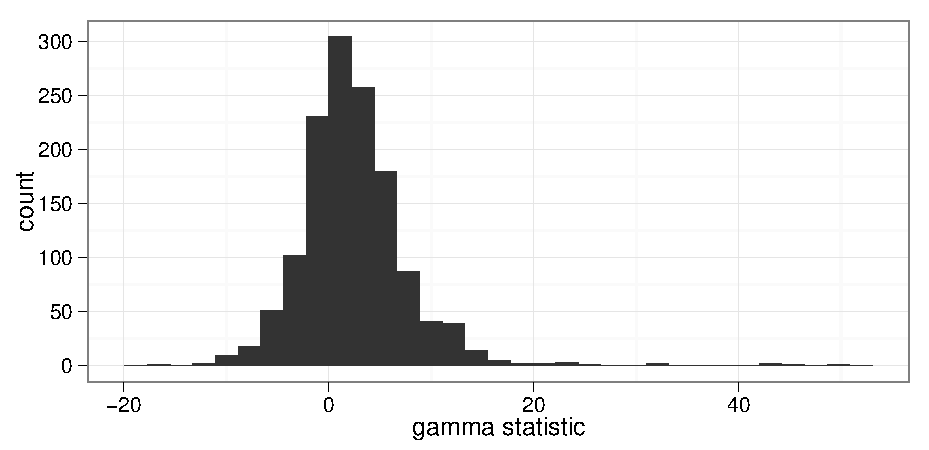
\includegraphics{figure2.pdf}
\caption{Distribution of the gamma statistic across phylogenies in
TreeBASE. Strongly positive values are indicative of an increasing rate
of evolution (excess of nodes near the tips), very negative values
indicate an early burst of diversification (an excess of nodes near the
root).}
\end{figure}

\section{Conclusion}

While we have focused on examples that require no additional data beyond
the phylogeny, a wide array of methods combine this data with
information about the traits, geography, or ecological community of the
taxa represented. In such cases, we would need programmatic access to
the trait data as well as the phylogeny. The Dryad digital repository
(\href{http://datadryad.org}{http://datadryad.org}) is an effort in this
direction. While programmatic access to the repository is possible
through the \texttt{rdryad} package (Chamberlain, Boettiger, and Ram
2012), variation in data formatting must first be overcome before
similar direct access to the data is possible. Dedicated databases such
as FishBASE (\href{http://fishbase.org}{http://fishbase.org}) may be
another alternative, where morphological data can be queried for a list
of species using the \texttt{rfishbase} package (Boettiger 2011). The
development of similar software for programmatic data access will
rapidly extend the space and scale of possible analyses.

The recent advent of mandatory data archiving in many of the major
journals publishing phylognetics-based research (\emph{e.g.} Fairbairn
2010; Piwowar, Vision, and Whitlock 2011; Whitlock et al. 2010), is a
particularly promising development that should continue to fuel the
trend of submissions seen in Fig. 1. Accompanied by faster and more
inexpensive techniques of NextGen sequencing, and the rapid expansion in
phylogenetic applications, we anticipate this rapid growth in available
phylogenies will continue. Faced with this flood of data, programmatic
access becomes not only increasingly powerful but an increasingly
necessary way to ensure we can still see the forest for all the trees.

\section{Acknowledgements}

CB wishes to thank S. Price for feedback on the manuscript, the TreeBASE
developer team for building and supporting the repository, and all
contributers to TreeBASE. CB is supported by a Computational Sciences
Graduate Fellowship from the Department of Energy under grant number
DE-FG02-97ER25308. The \texttt{treebase} package is is part of the
rOpenSci project (\href{http://ropensci.org}{ropensci.org}).

\section{References}

Blomberg, S. P., JR Theodore Garland, and A. R. Ives. 2003. ``Testing
for phylogenetic signal in comparative data: behavioral traits are more
labile.'' \emph{Evolution} 57: 717--745.

Boettiger, Carl. 2011. ``rfishbase.''
\href{http://cran.r-project.org/web/packages/rfishbase/}{http://cran.r-project.org/web/packages/rfishbase/}.

Boettiger, Carl, Graham Coop, and Peter Ralph. 2012. ``Is your phylogeny
informative? Measuring the power of comparative methods.''
\emph{Evolution} (Jan). doi:10.1111/j.1558-5646.2012.01574.x.

Butler, Marguerite A., and Aaron A. King. 2004. ``Phylogenetic
Comparative Analysis: A Modeling Approach for Adaptive Evolution.''
\emph{The American Naturalist} 164 (Dec): 683--695. doi:10.1086/426002.

Chamberlain, Scott, Carl Boettiger, and Karthik Ram. 2012. ``rdryad:
Dryad API interface.''
\href{http://www.github.com/ropensci/rdryad }{http://www.github.com/ropensci/rdryad
}.

Davies, T. Jonathan, Andrew P. Allen, Luís Borda-de-Água, Jim Regetz,
and Carlos J. Melián. 2011. ``Neutral biodiversity theory can explain
the imbalance of phylogenetic trees but not the tempo of their
diversification.'' \emph{Evolution} 65 (Jul): 1841--1850.
doi:10.1111/j.1558-5646.2011.01265.x.

Derryberry, Elizabeth P., Santiago Claramunt, Graham Derryberry, R.
Terry Chesser, Joel Cracraft, Alexandre Aleixo, Jorge Pérez-Emán, J. V.
Remsen Jr, and Robb T. Brumfield. 2011. ``Lineage diversification and
morphological evolution in a large-scale continental radiation: the
neotropical ovenbirds and woodcreepers (Aves: Furnariidae).''
\emph{Evolution} (Jul). doi:10.1111/j.1558-5646.2011.01374.x.

Drummond, Alexei J., and Andrew Rambaut. 2007. ``BEAST: Bayesian
evolutionary analysis by sampling trees.'' \emph{BMC evolutionary
biology} 7 (Jan): 214. doi:10.1186/1471-2148-7-214.

Eastman, Jonathan M., Michael E. Alfaro, Paul Joyce, Andrew L. Hipp, and
Luke J. Harmon. 2011. ``A novel comparative method for identifying
shifts in the rate of character evolution on trees.'' \emph{Evolution}
65 (Jul): 3578--3589. doi:10.1111/j.1558-5646.2011.01401.x.

Evans, Margaret E. K., Stephen A. Smith, Rachel S. Flynn, and Michael J.
Donoghue. 2009. ``Climate, niche evolution, and diversification of the
`bird-cage' evening primroses (Oenothera, sections Anogra and
Kleinia).'' \emph{The American Naturalist} 173 (Feb): 225--40.
doi:10.1086/595757.

Fairbairn, Daphne J. 2010. ``The Advent of Mandatory Data Archiving.''
\emph{Evolution} (Nov). doi:10.1111/j.1558-5646.2010.01182.x.

Fitzjohn, Richard G. 2010. ``Quantitative Traits and Diversification.''
\emph{Systematic Biology} 59 (Sep): 619--633. doi:10.1093/sysbio/syq053.

Gentleman, Robert, and Duncan Temple Lang. 2004. ``Statistical analyses
and reproducible research.'' \emph{Bioconductor Project Working Papers}:
2.

Goldberg, Emma E., Lesley T. Lancaster, and Richard H. Ree. 2011.
``Phylogenetic Inference of Reciprocal Effects between Geographic Range
Evolution and Diversification.'' \emph{Systematic Biology} 60 (May):
451--465. doi:10.1093/sysbio/syr046.

Harmon, Luke J., Jason T. Weir, Chad D. Brock, Richard E. Glor, and
Wendell Challenger. 2008. ``Geiger: investigating evolutionary
radiations.'' \emph{Bioinformatics} 24: 129--131.
doi:10.1093/bioinformatics/btm538.

Huelsenbeck, John P., and Fredrik Ronquist. 2001. ``MRBAYES: Bayesian
inference of phylogenetic trees.'' \emph{Bioinformatics} 17 (Aug):
754--5. doi:10.1093/bioinformatics/17.8.754.

Jombart, Thibaut, François Balloux, and Stéphane Dray. 2010. ``Adephylo:
New Tools for Investigating the Phylogenetic Signal in Biological
Traits.'' \emph{Bioinformatics} 26 (Aug): 1907--9.
doi:10.1093/bioinformatics/btq292.

Kembel, Steven W., Peter D. Cowan, Matthew R. Helmus, William K.
Cornwell, Helene Morlon, David D. Ackerly, Simon P. Blomberg, and
Campbell O. Webb. 2010. ``Picante: R tools for integrating phylogenies
and ecology.'' \emph{Bioinformatics} 26 (Jun): 1463--4.
doi:10.1093/bioinformatics/btq166.

Laubach, Thomas, and Arndt von Haeseler. 2007. ``TreeSnatcher: coding
trees from images.'' \emph{Bioinformatics} 23 (Dec): 3384--5.
doi:10.1093/bioinformatics/btm438.

Maddison, W. P., and D. R. Maddison. 2011. ``Mesquite: a modular system
for evolutionary analysis.''
\href{http://mesquiteproject.org}{http://mesquiteproject.org}.

Martins, E. P. 2004. ``COMPARE, version Computer programs for the
statistical analysis of comparative data.'' Bloomington IN.: Department
of Biology, Indiana University.
\href{http://compare.bio.indiana.edu/}{http://compare.bio.indiana.edu/}.

McPeek, Mark A., and Jonathan M. Brown. 2007. ``Clade age and not
diversification rate explains species richness among animal taxa.''
\emph{The American Naturalist} 169 (Apr): 97. doi:10.1086/512135.

McPeek, Mark a. 2008. ``The ecological dynamics of clade diversification
and community assembly.'' \emph{The American Naturalist} 172 (Dec): 270.
doi:10.1086/593137.

Morell, V. 1996. ``TreeBASE: the roots of phylogeny.'' \emph{Science}
273: 569. doi:10.1126/science.273.5275.569.

Paradis, Emmanuel. 2004. ``APE: Analyses of Phylogenetics and Evolution
in R language.'' \emph{Bioinformatics} 20: 289--290.
doi:10.1093/bioinformatics/btg412.

Parr, Cynthia S., Robert Guralnick, Nico Cellinese, and Roderic D. M.
Page. 2011. ``Evolutionary informatics: unifying knowledge about the
diversity of life.'' \emph{Trends in Ecology \& Evolution} 27 (Dec):
94--103. doi:10.1016/j.tree.2011.11.001.

Peng, R. D. 2011. ``Reproducible Research in Computational Science.''
\emph{Science} 334 (Dec): 1226--1227. doi:10.1126/science.1213847.

Phillimore, Albert B., and Trevor D. Price. 2008. ``Density-dependent
cladogenesis in birds.'' \emph{PLoS biology} 6 (Mar): 71.
doi:10.1371/journal.pbio.0060071.

Piwowar, Heather A., Todd J. Vision, and Michael C. Whitlock. 2011.
``Data archiving is a good investment.'' \emph{Nature} 473 (May):
285--285. doi:10.1038/473285a.

Pybus, O. G., and P. H. Harvey. 2000. ``Testing macro-evolutionary
models using incomplete molecular phylogenies.'' \emph{Proceedings of
The Royal Society B} 267 (Nov): 2267--72. doi:10.1098/rspb.2000.1278.

Quental, Tiago B., and Charles R. Marshall. 2010. ``Diversity dynamics:
molecular phylogenies need the fossil record.'' \emph{Trends in Ecology
\& Evolution} (Jun): 1--8. doi:10.1016/j.tree.2010.05.002.

R Development Core Team, The. 2012. ``R: A language and environment for
statistical computing.'' Vienna, Austria: R Foundation for Statistical
Computing. \href{http://www.r-project.org/}{http://www.r-project.org/}.

Rabosky, Daniel L. 2006. ``LASER: a maximum likelihood toolkit for
detecting temporal shifts in diversification rates from molecular
phylogenies.'' \emph{Evolutionary bioinformatics online} 2 (Jan):
273--6.

Revell, Liam J., D. Luke Mahler, Pedro R. Peres-Neto, and Benjamin D.
Redelings. 2011. ``a New Phylogenetic Method for Identifying Exceptional
Phenotypic Diversification.'' \emph{Evolution} (Aug).
doi:10.1111/j.1558-5646.2011.01435.x.

Sanderson, M. J., M. J. Donoghue, W. Piel, and T. Eriksson. 1994.
``TreeBASE: a prototype database of phylogenetic analyses and an
interactive tool for browsing the phylogeny of life.'' \emph{American
Journal of Botany} 81: 183.

Schliep, Klaus Peter. 2010. ``phangorn: Phylogenetic analysis in R.''
\emph{Bioinformatics} 27 (Dec): 592--593.
doi:10.1093/bioinformatics/btq706.

Schwab, M., N. Karrenbach, and J. Claerbout. 2000. ``Making scientific
computations reproducible.'' \emph{Computing in Science \& Engineering}
2: 61--67.

Stadler, Tanja. 2011a. ``Simulating Trees with a Fixed Number of Extant
Species.'' \emph{Systematic Biology} (Apr). doi:10.1093/sysbio/syr029.

---------. 2011b. ``Mammalian phylogeny reveals recent diversification
rate shifts.'' \emph{Proceedings of the National Academy of Sciences}
2011 (Mar). doi:10.1073/pnas.1016876108.

Stamatakis, Alexandros. 2006. ``RAxML-VI-HPC: maximum likelihood-based
phylogenetic analyses with thousands of taxa and mixed models.''
\emph{Bioinformatics} 22 (Nov): 2688--90.
doi:10.1093/bioinformatics/btl446.

Sukumaran, Jeet, and Mark T. Holder. 2010. ``DendroPy: A Python Library
for Phylogenetic Computing.'' \emph{Bioinformatics} 26 (Apr):
1569--1571. doi:10.1093/bioinformatics/btq228.

Temple Lang, Duncan. 2012a. ``RCurl: General network (HTTP/FTP/...)
client interface for R.''
\href{http://cran.r-project.org/package=RCurl}{http://cran.r-project.org/package=RCurl}.

---------. 2012b. ``XML: Tools for parsing and generating XML within R
and S-Plus.''
\href{http://cran.r-project.org/package=XML}{http://cran.r-project.org/package=XML}.

Vos, R. A., Hilmar Lapp, William H. Piel, and Val Tannen. 2010.
``TreeBASE2: Rise of the Machines.'' \emph{Nature Precedings}.
doi:10101/npre.2010.4600.1.
\href{http://hdl.handle.net/10101/npre.2010.4600.1}{http://hdl.handle.net/10101/npre.2010.4600.1}.

Vos, Rutger A., James P. Balhoff, Jason A. Caravas, Mark T. Holder,
Hilmar Lapp, Wayne P. Maddison, Peter E. Midford, et al. 2012. ``NeXML:
Rich, Extensible, and Verifiable Representation of Comparative Data and
Metadata.'' \emph{Systematic Biology} 61 (Jul): 675--89.
doi:10.1093/sysbio/sys025.

Vos, Rutger A., Jason Caravas, Klaas Hartmann, Mark A. Jensen, and Chase
Miller. 2011. ``BIO::Phylo-phyloinformatic analysis using perl.''
\emph{BMC Bioinformatics} 12 (Jan): 63. doi:10.1186/1471-2105-12-63.

Warren, Dan L., Richard E. Glor, and Michael Turelli. 2008.
``Environmental niche equivalency versus conservatism: quantitative
approaches to niche evolution.'' \emph{Evolution} 62 (Nov): 2868--83.
doi:10.1111/j.1558-5646.2008.00482.x.

Webb, Campbell O., David D. Ackerly, and Steven W. Kembel. 2008.
``Phylocom: software for the analysis of phylogenetic community
structure and trait evolution.'' \emph{Bioinformatics} 24 (Sep):
2098--100. doi:10.1093/bioinformatics/btn358.

Whitlock, Michael C., Mark A. McPeek, Mark D. Rausher, Loren Rieseberg,
and Allen J. Moore. 2010. ``Data archiving.'' \emph{The American
Naturalist} 175 (Mar): 145--6. doi:10.1086/650340.

Xie, Yihui. 2012. ``knitr: A general-purpose package for dynamic report
generation in R.''
\href{http://yihui.name/knitr/}{http://yihui.name/knitr/}.

%\begin{sloppypar} % more room to wrap urls
%\bibliography{}
%\end{sloppypar}

\end{document}
